\documentclass[12pt, letterpaper, twoside]{article}
\usepackage[utf8]{inputenc}

\usepackage{graphicx} %Allows you to import images.
\usepackage{float} %Allows for control of float positions.
\usepackage{cite} %Allows cititions  
\usepackage[hyphens,spaces,obeyspaces]{url} %Allows for url references 
\usepackage[table]{xcolor}

% Header and Footer Stuff 
\usepackage{fancyhdr}
\pagestyle{fancy}
\fancyhead{}
\fancyfoot{}
\fancyfoot[R]{\thepage\ }
\renewcommand{\headrulewidth}{0pt}
\renewcommand{\footrulewidth}{0pt}


\title{\textbf{Tutorial on how to create and manage storage account on Microsoft Azure}}
\author{Mujtaba Ahmed Abbasi}
\date{February 2017}

\begin{document}
	
	\begin{titlepage}
		\clearpage\maketitle
		\thispagestyle{empty}
	\end{titlepage}
	

\setcounter{page}{1}
\pagenumbering{arabic}

\section*{\textbf{Contents}}
\begin{itemize}
	\item{\large{Requirements}} 
	\item{\large{Creating an Azure Blob Storage account}}
	\item{\large{Creating a container in that storage account}}
	\item{\large{Seeing what containers exist within the storage account}}
	\item{\large{Uploading data to that container}}
	\item{\large{Seeing items are inside of that container}}
	\item{\large{Deleting an item in that container}}
	\item{\large{Deleting the container}}
	\item{\large{Deleting the storage account}}
	\item{\large{Installing Java Development Kit (JDK)}}
\end{itemize}
\clearpage

\section*{\textbf{Requirements}}
\begin{itemize}
	\item{\large{Sign in for 30 day free trial account from Microsoft Azure subscription.}}
	\item{\large{Install the Java Development Kit (JDK)}}
	\item{\large{Text editor, I will be using sublime 3}}
	
\end{itemize}
\clearpage

	
	
\section*{i. Creating an Azure Blob Storage account}	
We will be creating blob storage account in this step to store our unstructured data as objects in Azure storage. \par
\vspace{0.5cm}
1. Sign in to the Azure portal. \par
\vspace{0.5cm}
2. On the Hub menu, select \textbf{New}, \textbf{Storage} and then \textbf{Storage account}.
\begin{figure}[H]
	\centering
	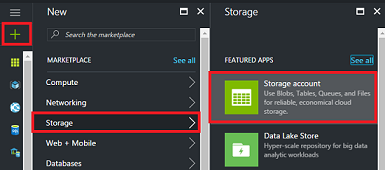
\includegraphics{/Users/azureimages/1}
\end{figure}
3. Enter a unique name for your storage account. Name must be of 3-24 \indent characters in length and may contain numbers and lowercase letters only. 
\begin{figure}[H]
	\centering
	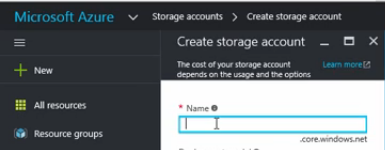
\includegraphics{/Users/azureimages/2}
\end{figure}
\clearpage
4. Select the deployment model option as \textbf{Resource Manager} . Blob \indent storage accounts can only be created using this particular option. 
\begin{figure}[H]
	\centering
	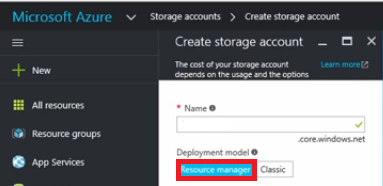
\includegraphics{/Users/azureimages/3}
\end{figure}
5. Change the type of storage account from General purpose to \textbf{Blob \indent Storage}. By default it is General purpose.
\begin{figure}[H]
	\centering
	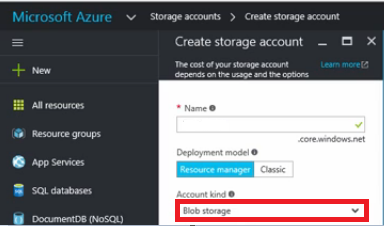
\includegraphics{/Users/azureimages/4}
\end{figure}
\clearpage
6. Now for \textbf{Performance} and \textbf{Replication} wise we will leverage the \indent default options for this demo.
\begin{figure}[H]
	\centering
	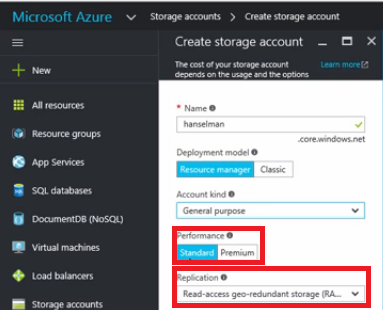
\includegraphics{/Users/azureimages/5}
\end{figure}
7. Leave the remaining fields default and hit the pin to dashboard button \indent at the bottom of your screen. Finally click the \textbf{Create} button to create \indent the storage account.  
\clearpage

\section*{ii. Creating a container in that storage account}	
In this step we will create a container (CloudBlobClient) in the storage account we created in the previous section. \par
\vspace{0.5cm}
1. Set a connection string to the Azure storage account. 
\begin{figure}[H]
	\centering
	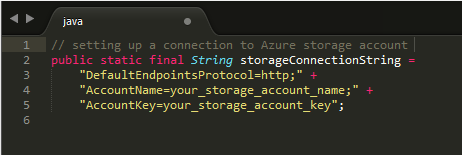
\includegraphics{/Users/azureimages/6}
\end{figure}
2. Create a container: Using \textbf{CloudBlobClient} we can get reference \indent objects for containers. You can create the container if it doesn't exist \indent with the \textbf{createIfNotExists} method, which will otherwise return the \indent existing container. 
\begin{figure}[H]
	\centering
	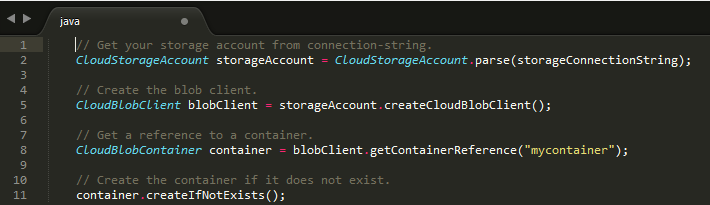
\includegraphics{/Users/azureimages/7}
\end{figure}
\clearpage

\section*{iii. Seeing what containers exist within the storage account}
In order to list the containers, we can use \textbf{ListContainers()} to list all containers in one storage account, consider the java code:
\begin{figure}[H]
	\centering
	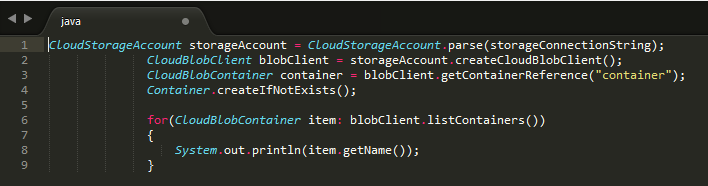
\includegraphics{/Users/azureimages/8}
\end{figure}
	
	
\section*{iv. Uploading data to that container}	
Now we have created a container, its time to upload data in it. Consider the code:
\begin{figure}[H]
	\centering
	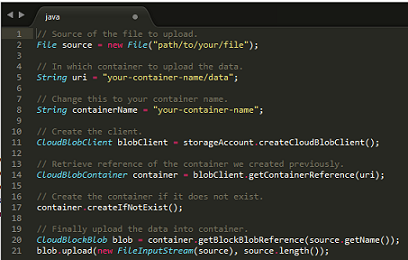
\includegraphics{/Users/azureimages/9}
\end{figure}
The above example will upload the data file into the data directory of \indent your container.

\section*{v. Seeing items are inside of that container}
To see the blobs in a container, we need to get reference of the container first like we did while uploading a blob. Using \textbf{listBlobs} method with a for loop, we can print the uri of each item in a container. Consider the java code:
\begin{figure}[H]
	\centering
	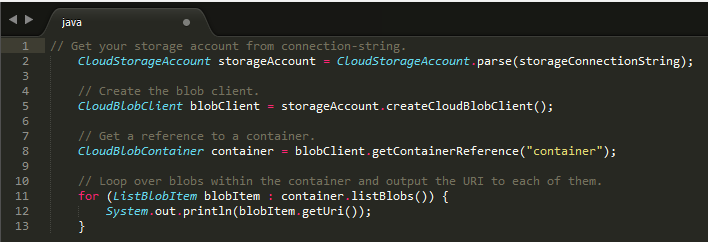
\includegraphics{/Users/azureimages/10}
\end{figure}
 		
\cleardoublepage 		
\section*{vi. Deleting an item in that container}
In order to delete an item, get a reference of that item and call \textbf{deleteIfExists}.
\begin{figure}[H]
	\centering
	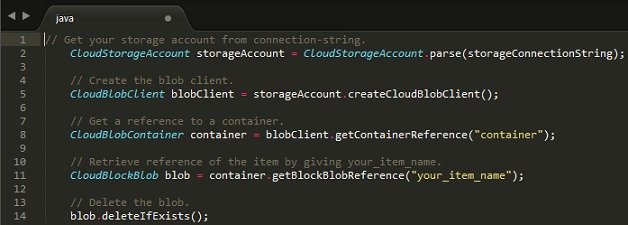
\includegraphics{/Users/azureimages/11}
\end{figure}
\section*{vii. Deleting the container}
To delete a blob container, consider the following code:
\begin{figure}[H]
	\centering
	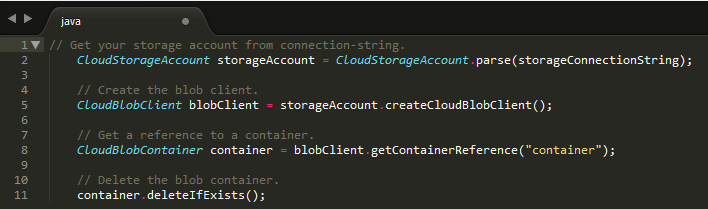
\includegraphics{/Users/azureimages/12}
\end{figure}
\vspace{1cm}
 \section*{viii. Deleting the storage account}	
 To delete storage account click the \textbf{Delete} button on top of your storage account in Azure portal. Deleting a storage account deletes the entire account, including all data in the account.	
\clearpage
\section*{Installing Java Development Kit (JDK)}
1. Go to \underline{http://www.oracle.com/technetwork/java/javase/downloads/index-jsp-138363.html} and select the highlighted box.
\begin{figure}[H]
	\centering
	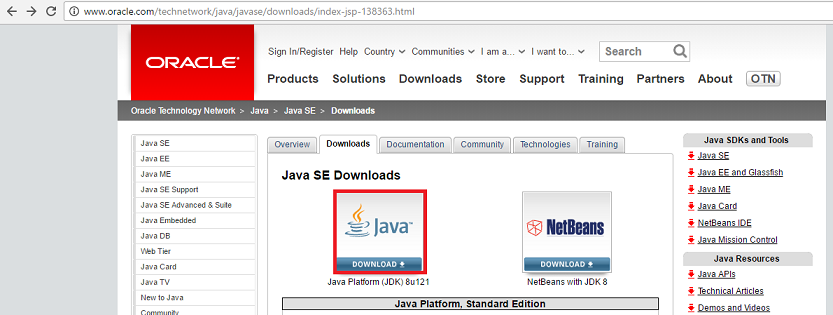
\includegraphics{/Users/azureimages/13}
\end{figure}
2. Select you preferred option and check the Accept license agreement, i am going for windows x84 depending upon my system specs.
\begin{figure}[H]
	\centering
	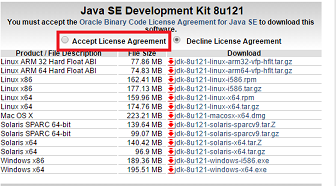
\includegraphics{/Users/azureimages/14}
\end{figure}
  		
 		
\end{document}